\chapter{Aplikacja mobilna}
Aplikacja stworzona w ramach pracy pozwala na konfigurację oraz komunikację z wcześniej opisanym robotem minisumo. Z racji, iż została napisana w natywnym języku \textit{Swift} wspieranym systemem operacyjnym jest system iOS.

\section{Kompatybilność}
Jedynym wymogiem, który musi zostać spełniony w celu uruchomienia aplikacji jest wersja systemu – nie starsza niż \textit{iOS 10}. W związku z czym aplikacja z powodzeniem powinna działać zarówno na tabletach oraz telefonach marki \textit{Apple} posiadających wspomnianą lub nowszą wersję systemu. 

Docelowo aplikacja była uruchamiana oraz testowana na urządzeniu \textit{iPhone 5}, który jest najstarszym telefonem wspierającym system iOS 10. Powodem wyboru urządzenia była optymalizacja, a mianowicie poprawność działania aplikacji na najsłabszych podzespołach gwarantowała odpowiednią pracę na mocniejszych jednostkach.

Dodatkowo poprawność wyświetlania oraz skalowania została przetestowana w symulatorze dostarczonym wraz z środowiskiem \textit{Xcode} na urządzeniach takich jak \textit{iPhone 6 Plus} oraz \textit{iPad Pro}.
 
\section{Wzorzec MVC}
Aplikacja mobilna została zaprojektowana została według wzorca architektonicznego MVC (z~ang. \textit{Model–View–Controller}), który często wykorzystywany jest do tworzenia interfejsów użytkownika. W omawianym wzorcu można wyróżnić trzy obiekty:
\begin{itemize}
\item model – odpowiada za serwowanie danych,
\item widok – odpowiada za wizualizację danych, 
\item kontroler – reaguje na poczynania użytkownika, zarządza odświeżeniem widoków oraz aktualizacją modelu. 
\end{itemize}
Podział opisanych ról przedstawiono na rysunku ~\ref{fig:mvc}.
\begin{figure}[H]
	\centering
		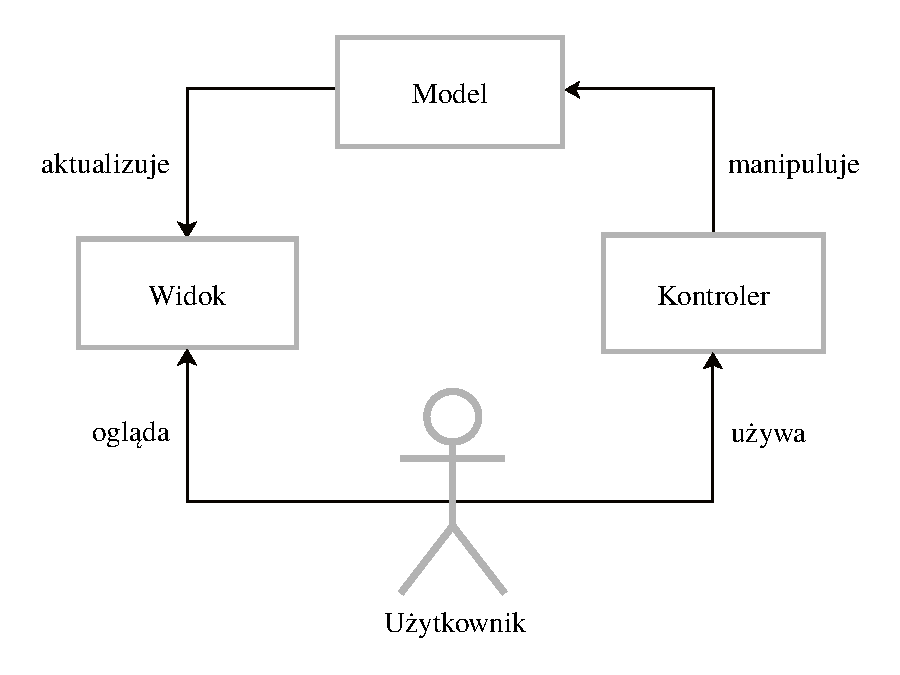
\includegraphics[width=0.75\linewidth]{pic05/mvc.pdf}
	\caption{Podział ról we wzorcu MVC.}
	\label{fig:mvc}	
\end{figure}

Dzięki wykorzystaniu tego wzorca uniezależniono przechowywane dane od sposobu w jaki są one przedstawiane użytkownikowi.

\section{Komunikacja}
Komunikacja z modułem Bluetooth została zrealizowana przy użyciu wcześniej wspomnianej platformy \textit{CoreBluetooth}. Utworzono klasę \textit{BluetoothSerial}, która była odpowiedzialna za całą logikę potrzebną do poprawnej wymiany danych między urządzeniami. Z racji, iż komunikacja jest nieodłącznym elementem każdej z funkcjonalności aplikacji skorzystano z protokołów. Protokoły są czymś na wzór intefejsów używanych w językach takich jak C++ bądź Java. Deklarują metody, lecz ich nie implementują. Każda klasa, która korzysta z komunikacji \textit{Bluetooth} musi zaimplementować metody zawarte w protokołach. Dzięki takiemu podejściu uniezależniamy logikę od kontrolerów. Klasa \textit{BluetoothSerial} nie jest w żaden sposób zależna od innych klas. Natomiast klasy, które wykorzystują komunikację, implementują odpowiednie metody w~zależności od indywidualnych konkretnych potrzeb.

\begin{minipage}{\textwidth}
	\begin{lstlisting}[label=protocolcode,caption=Protokół odpowiedzialny za komunikację między urządzeniami.]
protocol BluetoothSerialDelegate {
  func serialDidChangeState()
  func serialDidDisconnect(_ peripheral: CBPeripheral, error: NSError?)
  func serialDidReceiveString(_ message: String)
  func serialDidReadRSSI(_ rssi: NSNumber)
  func serialDidDiscoverPeripheral(_ peripheral: CBPeripheral, RSSI: NSNumber?)
  func serialDidConnect(_ peripheral: CBPeripheral)
  func serialDidFailToConnect(_ peripheral: CBPeripheral, error: NSError?)
  func serialIsReady(_ peripheral: CBPeripheral)
}
	\end{lstlisting}
\end{minipage}

Listing \ref{protocolcode} przedstawia zestaw metod zawartych w protokole komunikacyjnym.Poniżej przedstawiono przypadki w których zostają wywołane:

\begin{itemize}
\item \textit{serialDidChangeState} –  zmiana stanu modułu \textit{Bluetooth} (zostanie wyłączony lub włączony),
\item \textit{serialDidDisconnect} –  brak połączenia z modułem komunikacyjnym,
\item \textit{serialDidReceiveString} – została odebrana wiadomość typu tekstowego \textit{String},
\item \textit{serialDidReadRSSI} – gdy otrzymano sygnał RSSI (z ang. \textit{Received Signal Strength Indication}),
\item \textit{serialDidDiscoverPeripheral} – wykryto urządzenie podczas skanowania,
\item \textit{serialDidConnect} – połączono z urządzeniem, aczkolwiek urządzenie nie jest jeszcze gotowe na komunikację,
\item \textit{serialDidFailToConnect} – nie udało się nawiązać połączenia,
\item \textit{serialIsReady} – moduł jest gotowy na komunikację z aplikacją mobilną.
\end{itemize}

Tak jak wcześniej wspomniano, klasy korzystające z komunikacji mogą implementować dowolne z wyżej wymienionych metod w zależności od potrzeb.

\newpage

\section{Struktura aplikacji}
Tak jak wcześniej wspomniano, aplikacja została stworzona przy użyciu wzorca \textit{MVC}. Poniżej przedstawiono strukturę plików aplikacji.

\begin{figure}[H]
	\centering
		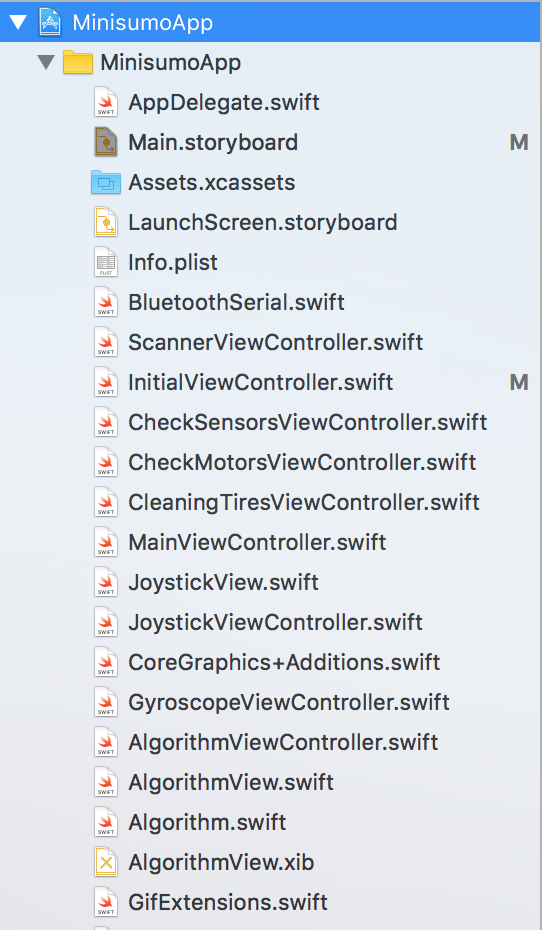
\includegraphics[width=0.75\linewidth, height=10cm, keepaspectratio]{pic05/structure.png}
	\caption{Struktura plików aplikacji mobilnej.}
	\label{fig:structure}	
\end{figure}

Na rysunku \ref{fig:structure} pliki o rozszerzeniu \textit{swift}, których nazwy kończą się na \textit{Controller} pełnią rolę kontrolerów, a \textit{View} widoków przedstawianych użytkownikowi. Reszta plików odpowiedzialna jest za logikę aplikacji. Dodatkowo plik \textit{Main.storyboard} zawiera konfiguracje większości widoków stworzonych przy użyciu graficznego narzędzia dostarczonego przez środowisko \textit{Xcode}.

\subsection{Panel powitalny}
Panel powitalny jest pierwszym widokiem z którym użytkownik ma do czynienia po uruchomieniu aplikacji mobilnej. Odpowiada on za poprawne wykrycie urządzenia \textit{Bluetooth} oraz dalszą komunikację. Składa się z elementów takich jak krótka instrukcja obsługi oraz przycisk \textit{Connect}, który po wciśnięciu wyświetla listę urządzeń gotowych na połączenie. Dodatkowo w przypadku wyłączonej komunikacji \textit{Bluetooth} zostanie wyświetlony komunikat o konieczności jej włączenia. 

\newpage

Po lewej stronie na obrazku \ref{fig:initial} przedstawiono omawiany panel, natomiast zdjęcie \ref{fig:scanner} po prawej stronie przedstawia listę dostępnych urządzeń.

\begin{figure}[H]
\centering
\begin{minipage}{.5\textwidth}
  \centering
  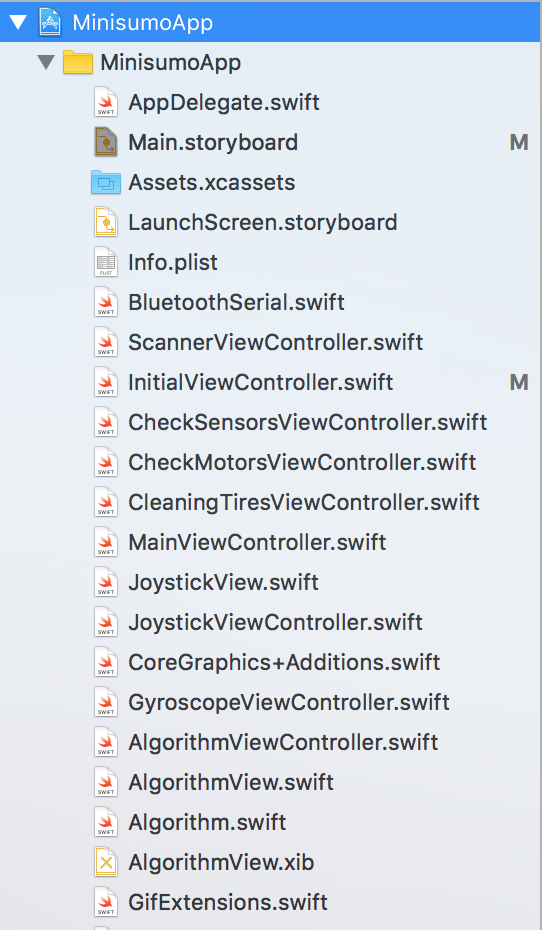
\includegraphics[width=.75\linewidth, height=10cm, keepaspectratio]{pic05/structure.png}
  \caption{Widok połączenia.}
  \label{fig:initial}
\end{minipage}%
\begin{minipage}{.5\textwidth}
  \centering
  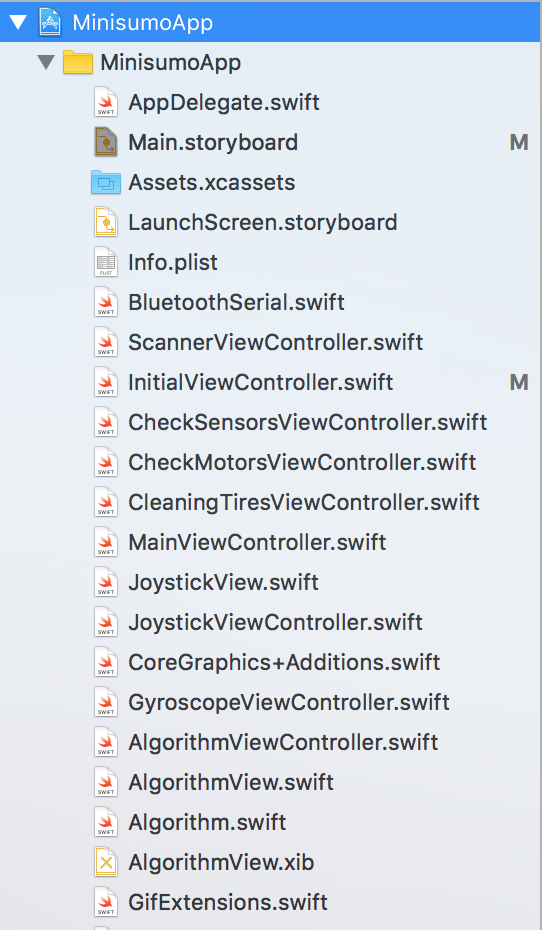
\includegraphics[width=.75\linewidth, height=10cm, keepaspectratio]{pic05/structure.png}
  \caption{Widok dostępnych urządzeń.}
  \label{fig:scanner}
\end{minipage}
\end{figure}

Za obsługę panelu powitalnego odpowiedzialna jest klasa \textit{InitialViewController}, która inicjalizuje globalny obiekt \textit{serial} , wykorzystywany do komunikacji \textit{Bluetooth} w obrębie całej aplikacji. Zdecydowano się na taki krok, ponieważ transmisja danych jest nieodłącznym elementem każdej funkcjonalności aplikacji, przez co uniknięto problemu z przekazywaniem obiektu pomiędzy kontrolerami.

\begin{minipage}{\textwidth}
	\begin{lstlisting}[label=scannerprotocol,caption=Implementacja protokołu.]
func serialDidDiscoverPeripheral(_ peripheral: CBPeripheral, RSSI: NSNumber?) {
  for exisiting in peripherals {
     if exisiting.peripheral.identifier == peripheral.identifier { return }
  }
    let theRSSI = RSSI?.floatValue ?? 0.0
    peripherals.append(peripheral: peripheral, RSSI: theRSSI)
    peripherals.sort { $0.RSSI < $1.RSSI }
    tableView.reloadData()
}
  
func serialDidFailToConnect(_ peripheral: CBPeripheral, error: NSError?) {
  tryAgainButton.isEnabled = true
}
  
func serialDidDisconnect(_ peripheral: CBPeripheral, error: NSError?) {
  tryAgainButton.isEnabled = true
}
  
func serialIsReady(_ peripheral: CBPeripheral) {
  performSegue(withIdentifier: "ShowMainViewController", sender: nil)
}
  
func serialDidChangeState() {
   if serial.centralManager.state != .poweredOn {
     dismiss(animated: true, completion: nil)
   }
}
	\end{lstlisting}
\end{minipage}

Listing \ref{scannerprotocol} przedstawia implementację metod zawartych w protokole \textit{BluetoothSerialDelegate} (omówionym w rozdziale 5.3) dla klasy \textit{ScannerViewController} odpowiedzialnej za wyświetlenie wykrytych urządzeń oraz poprawne połączenie z wybranym urządzeniem. Metoda \textit{serialDidDiscoverPeripheral} agreguje wykryte urządzenia, a następnie wysyła do widoku żądanie o wyświetleniu posortowanej listy ze znalezionymi urządzeniami. Funkcje \textit{serialDidFailToConnect} oraz \textit{serialDidDisconnect} odpowiedzialne są za przypadek, gdy nie udało się ustanowić połączenia z modułem \textit{Bluetooth} – wyświetlają przycisk dzięki któremu możliwa jest ponowna próba połączenia. Gdy aplikacja mobilna poprawnie ustanowiła połączenie z którymś z urządzeń uruchamiana jest funkcja \textit{serialIsReady}, której wynikiem jest przejście do panelu głównego.  Natomiast w przypadku rozłączenia wywoływana jest metoda \textit{serialDidChangeState} która wywołuje powrót do poprzedniego widoku jakim jest widok powitalny.

\subsection{Panel główny}
Panel główny odpowiedzialny jest tylko i wyłącznie za nawigację do poszczególnych funkcjonalności aplikacji. Składa się z prostego kontrolera \textit{MainViewController}, który nawiguje do odpowiednich paneli w zależności od wciśniętego przycisku.

\begin{figure}[H]
	\centering
		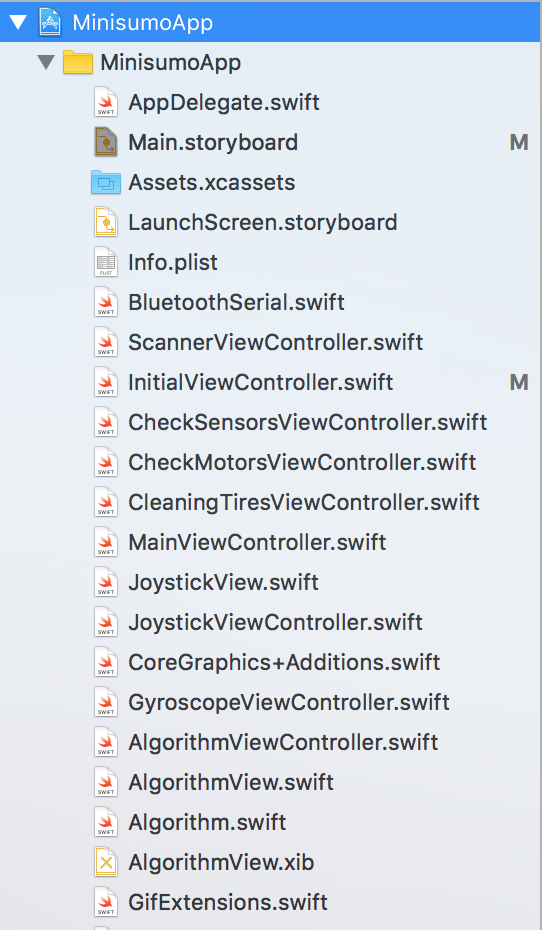
\includegraphics[width=0.75\linewidth, height=10cm, keepaspectratio]{pic05/structure.png}
	\caption{Panel główny aplikacji mobilnej.}
	\label{fig:mainview}	
\end{figure}

Na obrazku \ref{fig:mainview} przedstawiono wygląd panelu głównego aplikacji. Można zauważyć trzy przyciski \textit{Automatic}, \textit{Manual}, \textit{Pitstop}, które nawigują odpowiednio do panelu sterowania automatycznego, zdalnego oraz diagnostyki. 

\subsection{Panel sterowania automatycznego}
Panel sterowania automatycznego został stworzony w celu testowania algorytmów walki oraz konfigurowania robota do zawodów. Zaprojektowano go tak, aby był jak najbardziej intuicyjny w użytkowaniu. W górnej części widoku umiejscowione zostało zdjęcie formatu \textit{.gif} przedstawiające zachowanie robota na ringu dla danego algorytmu. Poniżej wizualizacji znajduje się krótki opis działania strategii, okno do ustawienia maksymalnej procentowej mocy silników oraz przełącznik, który określa czy robot powinien czekać na sygnał startowy (opcja wymagana podczas większości zawodów. Jej celem jest zapewnienie równego startu walczących ze sobą robotów). Na dole znajduje się przycisk \textit{START}, który po wciśnięciu wysyła do robota wiadomość z konfiguracją. Przerwanie walki następuje po wciśnięciu przycisku \textit{STOP} (który jest widoczny gdy wciśnięto przycisk \textit{START}).  W celu zmiany algorytmu należy przesunąć ekran od prawej do lewej lub na odwrót. Na samym dole znajdują się kropki odpowiadające każdemu z algorytmów, a najjaśniejsza z nich sygnalizuje, która strategia jest obecnie konfigurowana.

Zdjęcie \ref{fig:automaticview} ukazuje wygląd opisywanego panelu sterowania automatycznego. 

\begin{figure}[H]
	\centering
		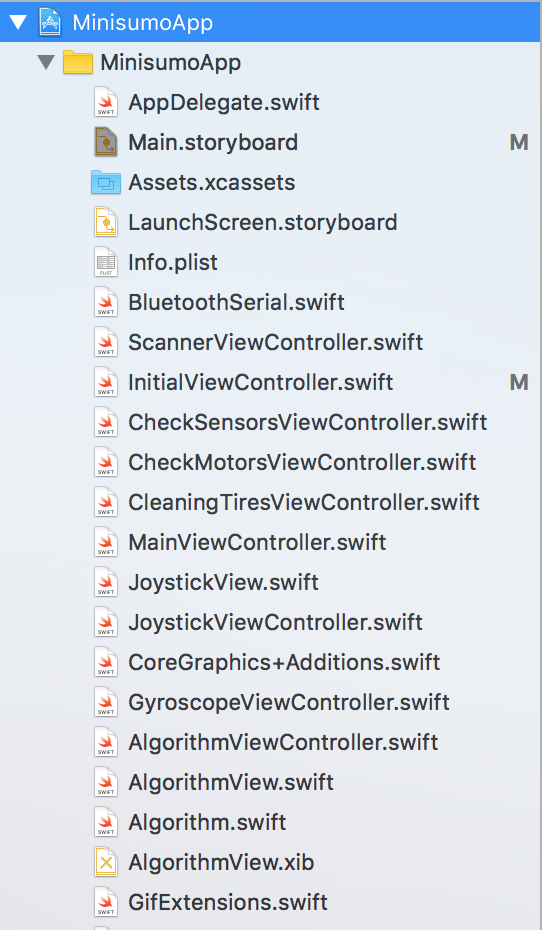
\includegraphics[width=0.75\linewidth, height=10cm, keepaspectratio]{pic05/structure.png}
	\caption{Panel sterowania automatycznego aplikacji mobilnej.}
	\label{fig:automaticview}	
\end{figure}

Za obsługę panelu sterowania automatycznego  odpowiada klasa 	\textit{AlgorithmViewController}, która wszystkie algorytmy walki przechowuje w tablicy \textit{algorithms} w postaci obiektów klasy \textit{Algorithm}.
  
\begin{minipage}{\textwidth}
	\begin{lstlisting}[label=algorithmclass,caption=Klasa Algorithm.]
class Algorithm {
  var description = ""
  var videoName = ""
  var isCompetition = false
}
	\end{lstlisting}
\end{minipage}

Listing \ref{algorithmclass} przedstawia klasę \textit{Algorithm}, która zawiera pola typu tekstowego \textit{description}, \textit{videoName} oraz logicznego \textit{isCompetition} odpowiadające odpowiednio opisowi działania algorytmu walki, ścieżce zdjęcia \textit{.gif} obrazującego zachowanie robota oraz informacji odnośnie tego czy robot powinien oczekiwać na sygnał startowy.
 
\subsection{Panel sterowania zdalnego}
Panel sterowania zdalnego pozwala na zdalne sterowanie silnikami robota za pomocą akcelerometru bądź wirtualnego dżojstiku. podobnie jak panel główny, posiada  widok z dwoma przyciskami, który nawiguje do poszczególnych funkcjonalności:
 
\subsubsection{Sterowanie akcelerometrem}
Sterowanie akcelerometrem pozwala na zdalne sterowaniem ruchem robota poprzez odpowiednie przechylenie telefonem. Sam panel składa się z krótkiej instrukcji obsługi, informacji o mocy oraz kierunku jazdy oraz przycisku \textit{START}, który służy do uruchomienia omawianej funkcjonalności.


Zdjęcie \ref{fig:accview} przedstawia wygląd omawianego panelu. Warto zauważyć, iż dla wygody został on zaprojektowany w orientacji poziomej.

\begin{figure}[H]
	\centering
		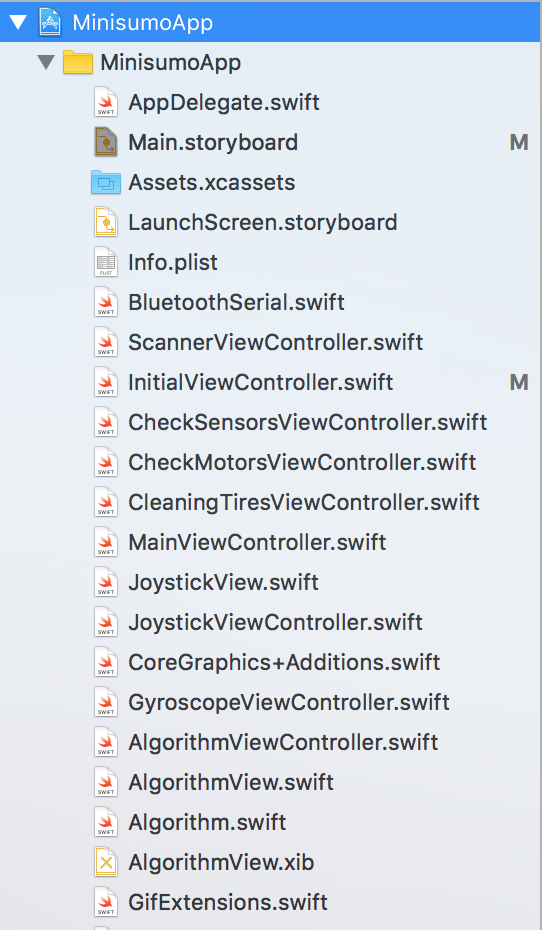
\includegraphics[width=0.75\linewidth, height=10cm, keepaspectratio]{pic05/structure.png}
	\caption{Panel sterowania zdalnego akcelerometrem.}
	\label{fig:accview}	
\end{figure}

W celu realizacji wyżej wspomnianej funkcjonalności wykorzystano obrót urządzenia wokół osi Y oraz Z. Obrót wokół osi Y odzwierciedla ruch robota w przód oraz w tył, natomiast obrót wokół osi Z kierunek ruchu – lewo lub prawo. Im większe wychylenie tym większa prędkość lub mocniejszy skręt. Dla lepszego zobrazowania problemu na rysunku \ref{fig:axis} przedstawiono orientację urządzenia.

\begin{figure}[H]
	\centering
		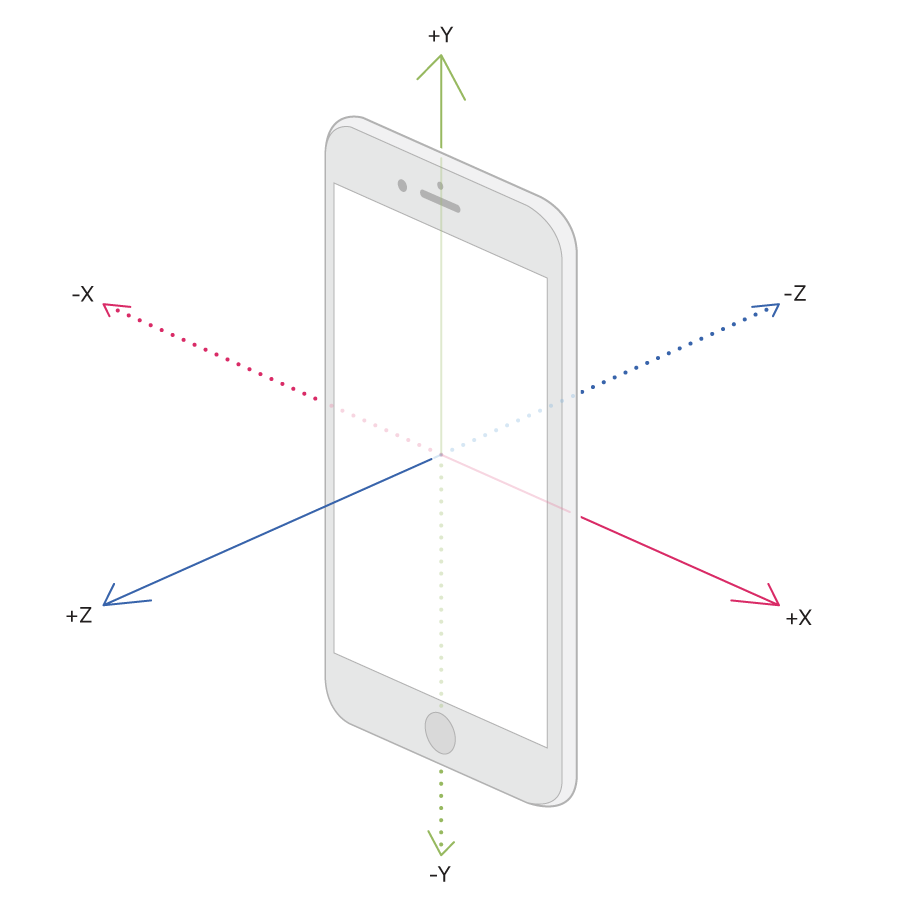
\includegraphics[width=0.6\linewidth]{pic05/axis}
	\caption{Osie X, Y oraz Z określające orientację urządzenia.}
	\label{fig:axis}	
\end{figure}

Listing \ref{accfunc} przedstawia fragment kodu, należący do klasy \textit{GyroscopeViewController}, a dokładniej metodę \textit{startAcc}, która zostaje wywołana w momencie wciśnięcia przycisku \textit{START}. Linia 2 ustawia czas, co który będzie zczytywany pomiar wychylenia urządzenia (w tym przypadku pomiar dokonywany jest co 200 milisekund). Następne zostaje uruchomiony akcelerometr oraz przechwytywane są wartości obrotów wokół wspomnianych wcześniej osi. Ich wartości zawierają się w zakresie od -1 do 1. Na ich podstawie określany jest kierunek oraz prędkość, które zostaną wysłane do robota.

\begin{minipage}{\textwidth}
	\begin{lstlisting}[label=accfunc,caption=Implementacja metody startAcc.]
func startAcc() {
  motionManager.deviceMotionUpdateInterval = 0.2
  motionManager.startDeviceMotionUpdates(to: OperationQueue.current!) { (data, error) in
  if let motion = data {
    var turn = Int(100 * motion.attitude.pitch)
    var power = Int(100 * motion.attitude.roll)
    
    . . . 

  }
   . . . 
}
	\end{lstlisting}
\end{minipage}

\subsubsection{Sterowanie wirtualnym dżojstikiem}
Sterowanie odbywa się za pomocą dwuwymiarowego drążka w postaci niebieskiego koła. Wychylenie drążka wpływa na kierunek jazdy oraz prędkość kół konstrukcji (im większe wychylenie tym większa prędkość). Dzięki zastosowaniu takiego rozwiązania możliwa jest jazda w przód oraz w tył. Dodatkowo w górnej części widoku znajduje się informacja odnośnie kierunku jazdy, wyrażonej kątowo w stopniach oraz mocy silników wyrażonej procentowo. Warto dodać, iż po puszczeniu drążka wraca on do początkowego położenia, które jest jednoznaczne z brakiem ruchu robota.

\begin{figure}[H]
	\centering
		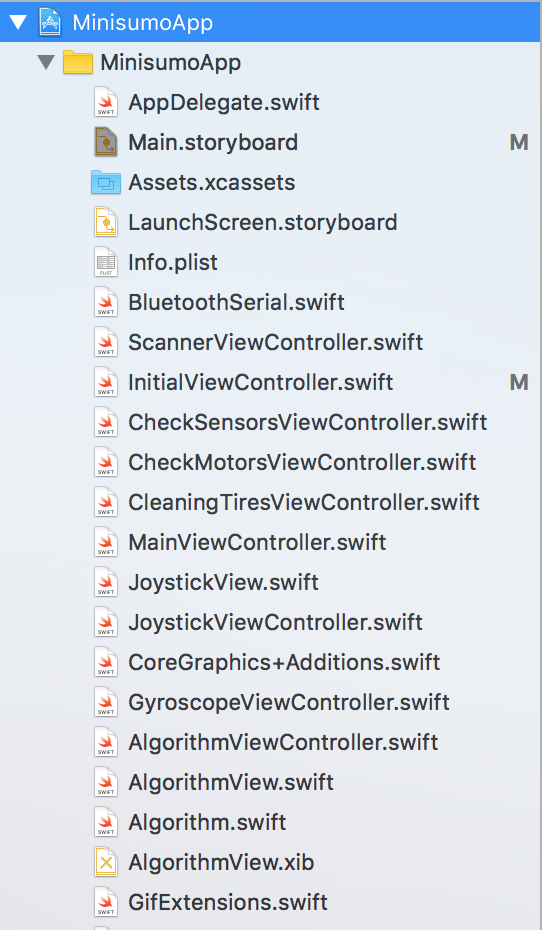
\includegraphics[width=0.75\linewidth, height=10cm, keepaspectratio]{pic05/structure.png}
	\caption{Panel sterowania zdalnego dżojstikiem.}
	\label{fig:joystickview}	
\end{figure}

Powyższe zdjęcie \ref{fig:joystickview} przedstawia wygląd panelu służącego do zdalnego sterowania robotem za pomocą dżojstiku.

\begin{figure}[H]
	\centering
		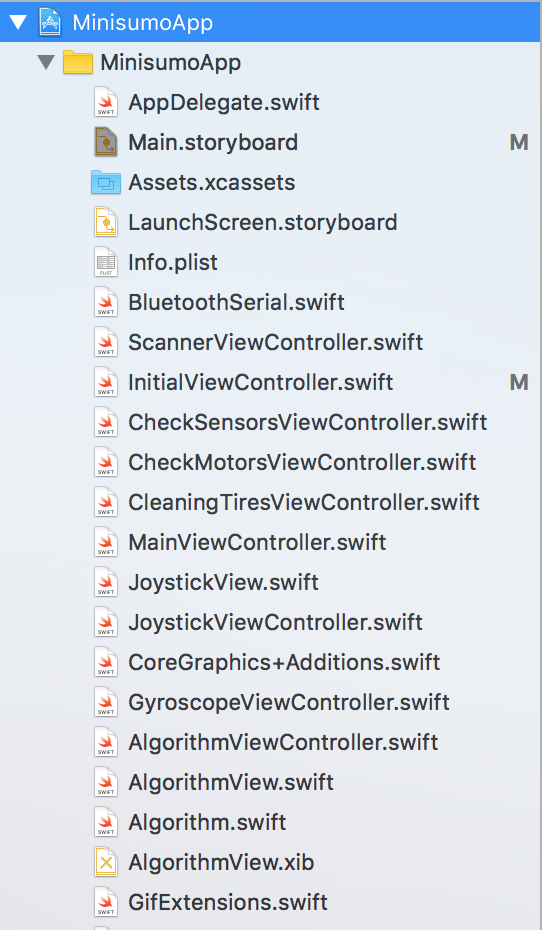
\includegraphics[width=0.75\linewidth, height=10cm, keepaspectratio]{pic05/structure.png}
	\caption{Wirtualny dżojstik.}
	\label{fig:joystickdirections}	
\end{figure}

Ilustracja \ref{fig:joystickdirections} przedstawia zależność kierunku jazdy konstrukcji od kąta odchylenia drążka. Jak łatwo zauważyć, górna półkula odpowiedzialna jest za jazdę w przód, natomiast dolna w tył (półkule zostały oddzielone czerwoną kreską). Analogicznie lewa półkula pozwala na jazdę w~lewo, a prawa w prawo (półkule zostały oddzielone zieloną kreską). Dodatkowo w celu ułatwienia oszacowania żądanej mocy silników utworzono okrąg, który wyznacza granicę maksymalnego wychylenia drążka.

Za zdalne sterowanie wirtualnym dżojstikiem odpowiedzialna jest klasa \textit{JoystickView}, (implementuje wygląd oraz położenie drążka) oraz klasa  \textit{JoystickViewController}, która nasłuchuje zmian położenia drążka oraz wysyła odpowiednią informację do robota. 

\begin{minipage}{\textwidth}
	\begin{lstlisting}[label=joystickcontrol,caption=Metoda klasy JoystickViewController.]
override func viewWillAppear(_ animated: Bool) {
    
   super.viewWillAppear(animated)
   serial.delegate = self
   msg[0] = "5"
   let rect = view.frame
   let size = CGSize(width: 150.0, height: 150.0)
   let joystick1Frame = CGRect(origin: CGPoint(x: rect.width/2 - size.width/2, y: rect.height/2), size: size)
   let joystick1 = JoyStickView(frame: joystick1Frame)
    
   view.addSubview(joystick1)
   joystick1.movable = false
   joystick1.alpha = 1.0
   joystick1.baseAlpha = 0.5 
   joystick1.handleTintColor = UIColor.blue
    
   joystick1.monitor = { angle, displacement in
     let power = Int(100 * displacement)
     let direction = Int(angle)

     self.leftTheta.text = "\(direction)"
     self.leftMagnitude.text = "\(power) %"
	
	 . . .
	
     usleep(useconds_t(20 * self.ms))
     serial.sendMessageToDevice(self.msg.joined())
   }
}  
	\end{lstlisting}
\end{minipage}

Powyższy listing \ref{joystickcontrol} przedstawia implementajcę najważniejszej funkcji klasy \textit{JoystickViewController}, którą jest \textit{viewWillAppear}. Jest to funkcja dostarczona przez platformę \textit{UIViewController} automatycznie wywoływana po załadowaniu widoku. Linia 5 przedstawia ustawienie pierwszego znaku wiadomości, która informuje robota jaka funkcjonalność powinna zostać obsłużona. Linie 6 – 15 ukazują konfigurację wyglądu dżojstiku, natomiast linia 17 deklaruje nasłuchiwanie zmian położenia drążka, które zwraca zmienne typu \textit{float}: \textit{angle} oraz \textit{displacement}, określające kąt (zakres 0 – 360 stopni) oraz wysunięcie (wartość od 0 do 1) drążka. Linia 18 skaluje wartość wysunięcia tak, aby wartość mieściła się w przedziale 0 – 100, co jest podyktowane wymogiem struktury wysyłanej wiadomości. Następnie w liniach 21 – 22 aktualizowane są informacje dostarczane użytkownikowi. Po odpowiednim przeliczeniu otrzymanych wartości na kierunki oraz moce silników następuje wysłanie wiadomości do robota (linia 27) poprzedzone 20 milisekundowym opóźnieniem (linia 26). Zastosowane opóźnienie spowodowane było ograniczoną przepustowością modułu \textit{Bluetooth} oraz niską wydajnością aplikacji. Dzięki opóźnieniu uzyskano pewność obsługi każdej wysłanej wiadomości kosztem niezauważalnego opóźnienia aktualizacji widoku przesunięcia drążka.

\subsection{Panel diagnostyki}
Panel diagnostyki powstał z myślą o sprawdzeniu poprawności działania poszczególnych komponentów robota. Niejednokrotnie zdarzało się, iż robot zachowywał się w nieoczekiwany sposób. Wtedy pojawiało się pytanie, czy wina leży po stronie oprogramowania, czy któryś z komponentów nie działa prawidłowo. Dzięki panelowi diagnostyki uzyskano możliwość szybszego zdiagnozowania problemu. 
Stworzony widok składa się z trzech zakładek: . Nawigowanie między funkcjonalnościami odbywa się za pomocą kliknięcia jednej z zakładek widocznych u dołu ekranu. 

\begin{figure}[H]
	\centering
		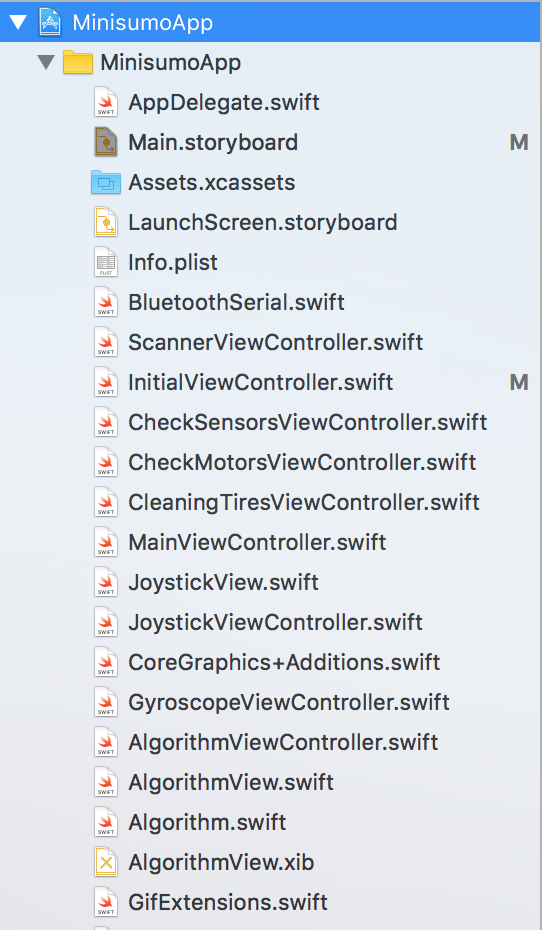
\includegraphics[width=0.75\linewidth, height=10cm, keepaspectratio]{pic05/structure.png}
	\caption{Widok zakładek w panelu diagnostyki.}
	\label{fig:pitstopview}	
\end{figure}

Rysunek \ref{fig:pitstopview} przedstawia zakładki nawigujące do poszczególnych opcji diagnostycznych.

\newpage

\subsubsection{Diagnostyka czujników}
Panel diagnostyki czujników powstał z myślą o sprawdzeniu poprawności działania czterech czujników wykrywających przeciwnika. Po włączeniu tego widoku zostaje wysłana wiadomość do robota z żądaniem obsłużenia odpowiedniej funkcjonalności. Następnie co 20 milisekund robot wysyła informację zwrotną, zawierającą stan czujników. W przypadku, gdy któryś z czujników wykrył obiekt znajdujący się przed nim, na ekranie pojawia się etykieta \textit{work} w odpowiednim miejscu. Klasą odpowiedzialną za obsługę funkcjonalności jest \textit{CheckSensorsViewController}.

\begin{figure}[H]
	\centering
		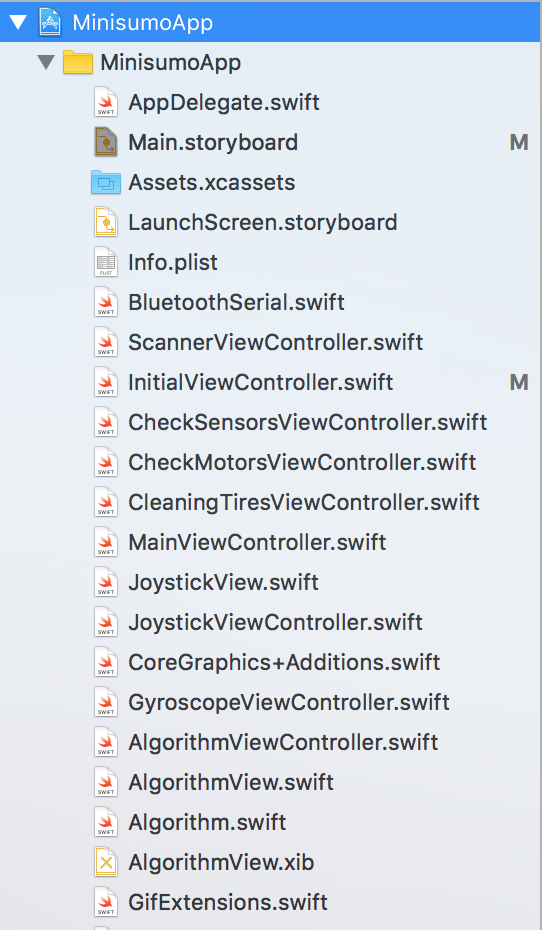
\includegraphics[width=0.75\linewidth, height=10cm, keepaspectratio]{pic05/structure.png}
	\caption{Widok diagnostyki czujników.}
	\label{fig:diagsensors}	
\end{figure}

Rysunek \ref{fig:diagsensors} ukazuje widok diagnostyki czujników. Przedstawiono na nim przypadek, gdzie każdy z czujników wykrył przeciwnika. Górne etykiety odpowiadają czujnikom znajdującym się w frontalnej części robota, natomiast boczne odpowiadają odpowiednio lewemu oraz prawemu czujnikowi.


\begin{figure}[H]
	\centering
		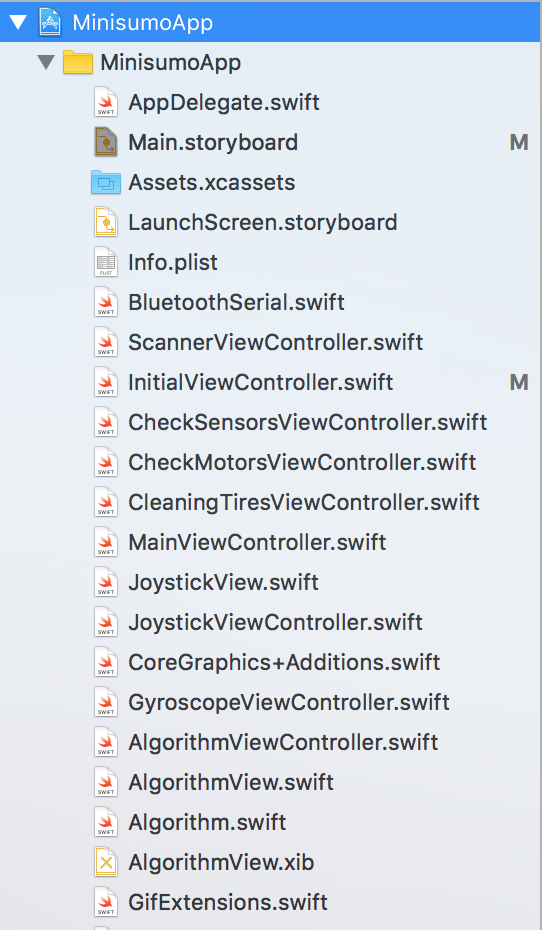
\includegraphics[width=0.75\linewidth, height=10cm, keepaspectratio]{pic05/structure.png}
	\caption{Poprawność działania diagnostyki czujników.}
	\label{fig:realsensors}	
\end{figure}

Natomiast na ilustracji \ref{fig:realsensors} przedstawiono działanie omawianego panelu. Po lewej stronie znajduje się robot z zasłoniętym lewym oraz górnym czujnikiem (oznacza to wykrycie przeciwnika), a po prawej stronie telefon z wizualizacją działania aplikacji. Jak widać wiadomość nadesłana z robota została odpowiednio zinterpretowana, ponieważ pojawiła się lewa oraz górna etykieta \textit{work}.

\begin{minipage}{\textwidth}
	\begin{lstlisting}[label=sensors,caption=Parsowanie wiadomości zawierającej stan czujników.]
func parseSensors(state: String, label: UILabel) {
  if state == "1" {
    label.text = "work"
  } else {
    label.text = " "
  }
}
	\end{lstlisting}
\end{minipage}

Powyższy listing \ref{sensors} przedstawia funkcję \textit{parseSensors}, która ma na celu interpretację fragmentu wiadomości odnośnie stanu czujników nadesłanej przez robota. W przypadku otrzymania wartości \textit{1} oznaczającej wykrycie przeciwnika pojawia się etykieta \textit{work}. W innych przypadkach etykieta jest niewidoczna.
 
\subsubsection{Diagnostyka silników}
Panel diagnostyki silników powstał w celu sprawdzenia zachowania poszczególnego motoru. Jego widok składa się z dwóch niezależnych suwaków, które służą do ustawienia odpowiedniej mocy oraz kierunku obrotu każdego z silników.

Obrazek \ref{fig:motors} przedstawia wygląd omawianego panelu. Domyślnie suwaki są wyśrodkowane, co oznacza brak obrotu. Przesunięcie suwaka w lewo powoduje obrót silnika w tył, natomiast w~prawo obrót w przód.

\begin{figure}[H]
	\centering
		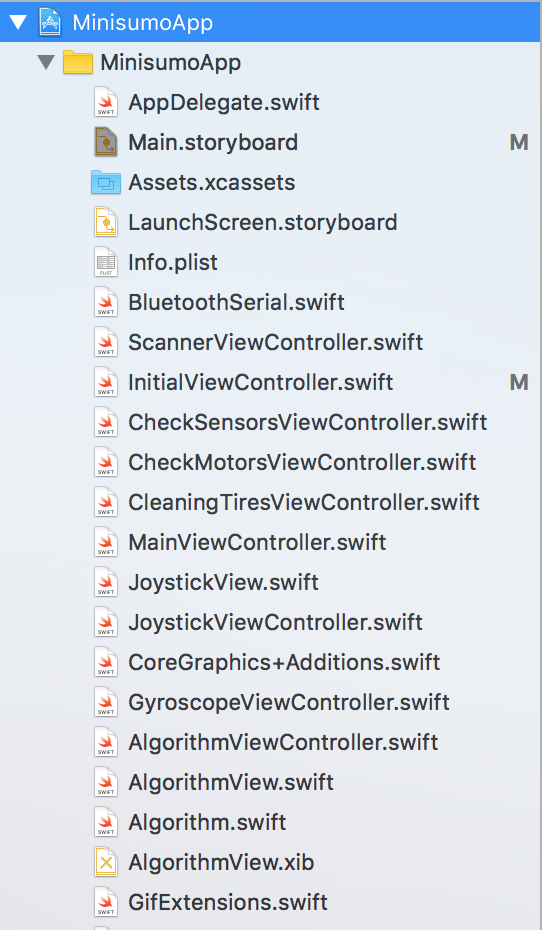
\includegraphics[width=0.75\linewidth, height=10cm, keepaspectratio]{pic05/structure.png}
	\caption{Widok diagnostyki silników.}
	\label{fig:motors}	
\end{figure}

Listing \ref{motorscode} zawiera implementację metody \textit{RightMotor} (należącej do klasy \textit{CheckMotorsViewController}), która nasłuchuje zmian położenia suwaka. Zakres wartości mieści się w przedziale od -100 do 100, gdzie wartości ujemne interpretowane są jako obrót silnika w tył (przeciwnie do ruchu wskazówek zegara). Linia 3 przedstawia pobranie wartości położenia suwaka. Linie 4 – 9 ukazują fragment kodu, który parsuje uzyskaną wartość i określa kierunek obrotu. Następnie wartość położenia suwaka jest parsowana na pojedyncze znaki oraz przypisywana do odpowiednich indeksów tablicy \textit{msg}, która zostaje wysłana do robota. Wiadomość z żądaną mocą oraz kierunkiem obrotu silnika wysyłana jest co 200 milisekund z powodów opisanych w~poprzednich podrozdziałach pracy. Analogicznie dla lewego silnika powstała metoda \textit{LeftMotor}.

\begin{minipage}{\textwidth}
	\begin{lstlisting}[label=motorscode,caption=Nasłuchiwanie zmiany położenia suwaka.]
IBAction func RightMotor(_ sender: UISlider) {
  
  rightMotorPower = Int(sender.value)
  if rightMotorPower < 0 {
    rightMotorDirection = 1
    rightMotorPower *= -1
  } else {
    rightMotorDirection = 2
  }
    
  msg[2] = String(rightMotorDirection)
    
  if rightMotorPower < 10 {
    msg[5] = "0"
    msg[6] = String(rightMotorPower)
  } else {
    msg[5] = String(rightMotorPower / 10)
    msg[6] = String(rightMotorPower % 10)
  }
    
  usleep(useconds_t(20 * ms))
  print(msg.joined())
  serial.sendMessageToDevice(msg.joined())
}
	\end{lstlisting}
\end{minipage}

\subsubsection{Czyszczenie opon}
Panel czyszczenia opon jest uboższą wersją panelu diagnostyki silników. Składa się z jednego przełącznika, który ustala moc obu silników na 20\% dostępnej mocy. Funkcjonalność powstała z myślą o czyszczeniu opon robota, które wykonane zostały z poliuretanu przez co bardzo szybko tracą przyczepność z powodu dużej podatności na zbieranie brudu.

\newpage

Poniższe zdjęcie \ref{fig:tires} przedstawia wygląd panelu służącemu czyszczenia opon konstrukcji.

\begin{figure}[H]
	\centering
		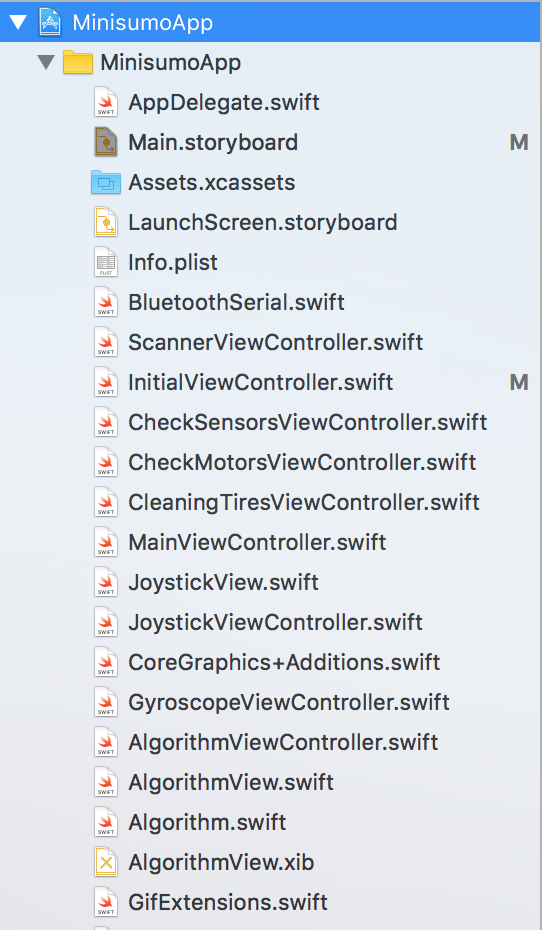
\includegraphics[width=0.75\linewidth, height=10cm, keepaspectratio]{pic05/structure.png}
	\caption{Widok funkcji czyszczenia opon.}
	\label{fig:tires}	
\end{figure}

Na listingu \ref{tirescode} przedstawiono metodę \textit{changedState} będącą członkiem klasy \textit{CleaningTiresViewController}. Wywoływana jest w momencie zmiany położenia przełącznika, a następnie w~zależności od jego stanu wysyła odpowiednio skonstruowaną wiadomość do robota.  

\begin{minipage}{\textwidth}
	\begin{lstlisting}[label=tirescode,caption=Nasłuchiwanie zmiany położenia przełącznika.]
IBAction func changedState(_ sender: UISwitch) {
  if sender.isOn {
    msg[0] = "3"
    serial.sendMessageToDevice(msg.joined())
  } else {
    msg[0] = "0"
    serial.sendMessageToDevice(msg.joined())
  }
}
	\end{lstlisting}
\end{minipage}

